
%%%%%%%%%%%%%%%%%%%%%%%%%%%%%%%%%%%%%%%%%%%%%%%%%%%%%%%%%%%%%%%%%%%%%%%%%%%%%
%%%%% Basic C++ %%%%%%%%%%%%%%%%%%%%%%%%%%%%%%%%%%%%%%%%%%%%%%%%%%%%%%%%%%%%%
%%%%%%%%%%%%%%%%%%%%%%%%%%%%%%%%%%%%%%%%%%%%%%%%%%%%%%%%%%%%%%%%%%%%%%%%%%%%%
\begin{frame}
\pointedsl{
	Basic C++
}
\end{frame}

%%%%%%%%%%%%%%%%%%%%%%%%%%%%%%%%%%%%%%%%%%%%%%%%%%%%%%%%%%%%%%%%%%%%%%%%%%%%%
\lstset{language=C++,numbers=none}
\begin{frame}[fragile]
\frametitle{Declaration and definition}
\begin{lstlisting}
void process(int x); // declare a function
int x; // declare a variable
x = 10; // assign a value
process(x);
// declaration and definition
int sum(int a, int b){ return a + b; }
// declaration and assignment
int y = sum(x, 2);
\end{lstlisting}
\misc{
	Every variable, type or function must be declared before being used. They can then be defined anywhere.
	
	\textbf{Note}: variables automatically receive a default value corresponding to $0$.
}
\end{frame}

%%%%%%%%%%%%%%%%%%%%%%%%%%%%%%%%%%%%%%%%%%%%%%%%%%%%%%%%%%%%%%%%%%%%%%%%%%%%%
\begin{frame}[fragile]
\frametitle{Flow control}
\begin{center}
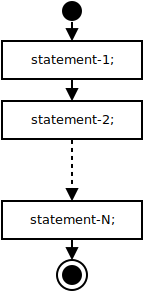
\includegraphics[width=0.7\textwidth]{figures/flow}
\end{center}
\misc{
	The usual conditional blocks are available
	\begin{itemize}
		\item \ctext{if}, \ctext{else if}, \ctext{else} and \ctext{switch}
	\end{itemize}
	as well as loop structures
	\begin{itemize}
		\item \ctext{for}, \ctext{while} and \ctext{do while}
	\end{itemize}
}
\end{frame}

%%%%%%%%%%%%%%%%%%%%%%%%%%%%%%%%%%%%%%%%%%%%%%%%%%%%%%%%%%%%%%%%%%%%%%%%%%%%%
\begin{frame}[fragile]
\frametitle{Arrays and pointers}
\begin{columns}[c]
  \begin{column}{0.5\textwidth}
\lstset{language=C++,numbers=left}
\begin{lstlisting}
int a[5];
a[0] = 1;
int *b = &a[0];
b += 3;
*b = 42;
b[1] = 5;
\end{lstlisting}
  \end{column}
  \begin{column}{0.5\textwidth}
    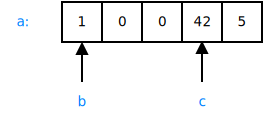
\includegraphics[width=0.7\textwidth]{figures/array.pdf}
  \end{column}
\end{columns}
\misc{
	\emph{Arrays} are continuous blocks of memory that store multiple elements of a same type (a fixed number of them!).
	
	\emph{Pointers} are a special type of variables that point to memory addresses.
}
\end{frame}

%%%%%%%%%%%%%%%%%%%%%%%%%%%%%%%%%%%%%%%%%%%%%%%%%%%%%%%%%%%%%%%%%%%%%%%%%%%%%
\begin{frame}[fragile]
\frametitle{Passing by value}
\begin{lstlisting}
void swap_wrong(int x, int y){
    int tmp = x;
    x = y;
    y = tmp;
}
int a = 1, b = 2;
swap_wrong(a, b);
// did not work! a=1, b=2
\end{lstlisting}
\misc{
	Function arguments are \textbf{passed by value} (copy of value). We need pointers to modify \ctext{a} and \ctext{b} in the code above.
}
\end{frame}

%%%%%%%%%%%%%%%%%%%%%%%%%%%%%%%%%%%%%%%%%%%%%%%%%%%%%%%%%%%%%%%%%%%%%%%%%%%%%
\begin{frame}[fragile]
\frametitle{Correct swap using pointers}
\begin{lstlisting}
void swap_ptr(int *x, int *y){
    int tmp = *x;
    *x = *y;
    *y = tmp;
}
int a = 1, b = 2;
swap_ptr(&a, &b);
// now a=2, b=1
\end{lstlisting}
\misc{
	\ctext{\&a} uses the \textbf{reference} operator to get the adresse of \ctext{a}.
	
	\ctext{*x} uses the \textbf{dereference} operator to get / set the value at the adress given by \ctext{x}.
}
\end{frame}

